% ==================================================================
%  Sujet 4 : Gravure de l'aluminium et alignement de masque
%  Seance du 9 novembre 2026, DLL-MED
% ==================================================================
\section{Gravure de l'aluminium et alignement de masque}

\subsection{Objectif}

\noindent Ce sujet vise à mettre en pratique deux étapes essentielles de la photolithographie : la gravure sélective d’une couche d’aluminium et l’alignement d’un photomasque sur des motifs préexistants \cite{intro,prot4}.

\noindent La première partie consiste à transférer des motifs sur une couche d’aluminium par photolithographie, suivie d’une gravure chimique humide. L’objectif est de déterminer le temps nécessaire à la gravure pour les deux types de chip utilisés : du verre et du silicium, en plus d’observer les motifs obtenus au microscope optique.

\noindent La seconde partie consiste à aligner précisément un photomasque avec des structures déjà présentes sur un wafer, afin de réaliser une nouvelle exposition UV et d'évaluer la qualité de l'alignement.

\subsection{Matériels}
Le matériel est listé au tableau~\ref{tab:s4-materiel}.

\begin{table}[htbp]
  \centering\small
  \caption{Matériel utilisé pendant la séance.}
  \label{tab:s4-materiel}
  \begin{tabularx}{\linewidth}{@{}lX@{}}
    \toprule
    \textbf{Catégorie} & \textbf{Utilisé pendant la séance} \\
    \midrule
    Équipements & chips en verre et silicium recouverts d'aluminium, wafer de silicium avec motifs, plaque chauffante, spin coater, aligneur de masque UV, photomasques, microscope optique, hotte chimique, béchers, pistolet à azote \\
    Produits chimiques & résine positive AZ1512 \cite{tdsaz1500}, révélateur AZ 726 MIF, solution de gravure de l'aluminium A (mélange d'acide acétique, nitrique et phosphorique), acétone, alcool isopropylique, eau déionisée (DI) \\
    \bottomrule
  \end{tabularx}
\end{table}


\subsection{Méthodes}

\subsubsection{Étapes expérimentales}

\noindent\textbf{A. Gravure de l'aluminium}

\begin{figure}[htbp]
    \centering
    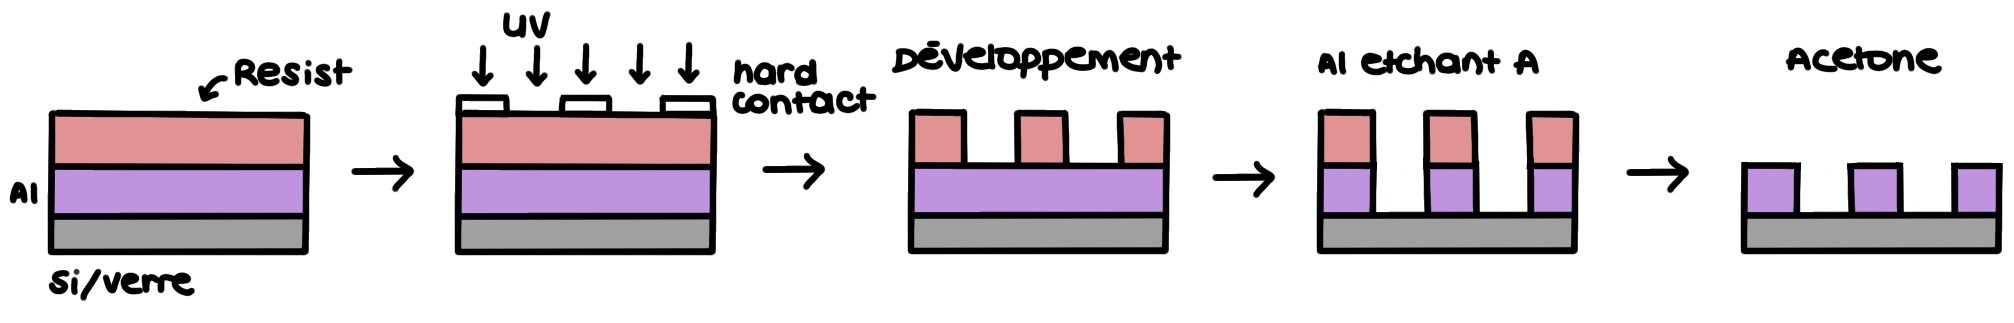
\includegraphics[width=\textwidth]{rapport-micro332/photos/s4_gravure_alu.jpg}
    \caption{Étapes de la gravure de l'aluminium}
    \label{fig:s4_gravure_aluminium}
\end{figure}

Pour chaque chip, en verre et en silicium, on suit les étapes de la figure~\ref{fig:s4_gravure_aluminium} :

\begin{enumerate}

    \item \textbf{Préparation du chip :}
    Le chip est déshydraté sur une plaque chauffante à \qty{150}{\celsius} pendant \qty{2}{\minute} (cette étape a été réalisée avant le début du TP). Une couche de résine positive AZ1512 est ensuite déposée par centrifugation, en deux étapes successives : \qty{700}{\tour\per\minute} pendant \qty{7}{\second}, puis \qty{4000}{\tour\per\minute} pendant \qty{60}{\second}. Un soft bake est réalisé à \qty{100}{\celsius} pendant \qty{60}{\second}.

    \item \textbf{Photolithographie :}
    Le chip est exposé aux UV à travers un photomasque pendant \qty{10}{\second}, en hard contact. La résine est ensuite développée dans une solution AZ 726 MIF pendant \qty{45}{\second}, sous agitation douce. Après un rinçage à l'eau DI pendant \qty{1}{\minute} et un séchage à l'azote, une cuisson supplémentaire (post-bake) est effectuée à \qty{100}{\celsius} pendant \qty{90}{\second} afin de durcir la résine restante.

    \item \textbf{Inspection initiale :}
    Les motifs obtenus sont observés au microscope optique et une image de référence est enregistrée.

    \item \textbf{Gravure chimique :}
    Le chip est immergé dans une solution Aluminum Etchant A, maintenue à \qty{40}{\celsius} et constituée d'acides phosphorique, nitrique et acétique ainsi que d'eau DI, dans un rapport volumique de 16:1:1:2. Le temps nécessaire à l'élimination complète de l'aluminium non protégé par la résine est mesuré pour les deux chips. Le chip est ensuite rincé successivement dans deux bains d'eau DI pendant \qty{3}{\minute} chacun, puis séché.

    \item \textbf{Inspection finale :}
    Les motifs gravés sont observés au microscope optique. La résine restante est ensuite retirée à l'acétone, suivie d'un rinçage à l'IPA et à l'eau DI.

\end{enumerate}

\noindent\textbf{B. Alignement du photomasque}

\begin{figure}[htbp]
    \centering
    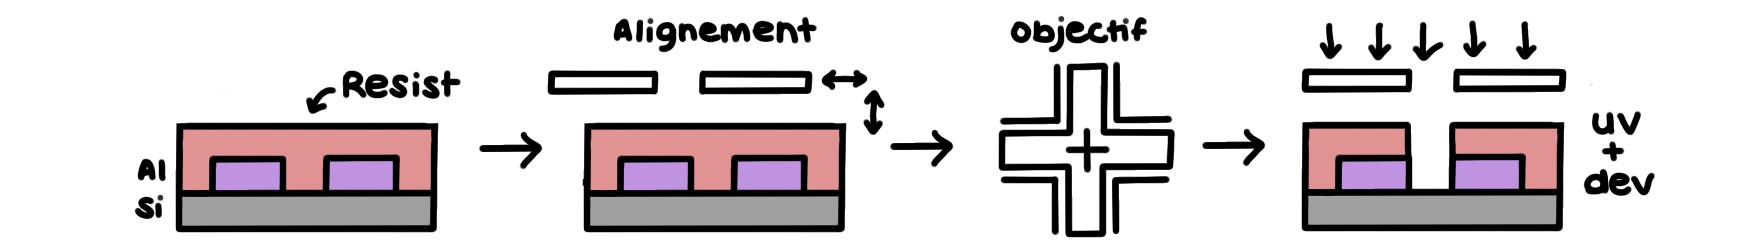
\includegraphics[width=\textwidth]{rapport-micro332/photos/s4_align_mask.jpg}
    \caption{Étapes de l'alignement de masque}
    \label{fig:s4_align_mask}
\end{figure}

De façon à positionner précisément les motifs d'un photomasque par rapport à des structures déjà présentes sur le wafer, on suit les étapes de la figure~\ref{fig:s4_align_mask} :

\begin{enumerate}

    \item \textbf{Préparation du wafer :}
    Le wafer est déshydraté à \qty{150}{\celsius} pendant \qty{5}{\minute} (cette étape a été réalisée avant le début du TP). La résine AZ1512 est déposée à \qty{700}{\tour\per\minute} pendant \qty{7}{\second}, puis à \qty{4000}{\tour\per\minute} pendant \qty{60}{\second}. Une précuisson à \qty{100}{\celsius} pendant \qty{60}{\second} est ensuite effectuée.

    \item \textbf{Mise en place :}
    Le wafer est placé au centre du support de l'aligneur et maintenu par aspiration. Le photomasque est fixé dans le support supérieur, avec sa face chromée orientée vers le wafer. Le wafer est progressivement rapproché du masque jusqu'à un léger contact permettant de rendre leurs surfaces parallèles. Le mécanisme de parallélisation est ensuite verrouillé.

    \item \textbf{Alignement :}
    Le wafer est abaissé afin d'établir un écart de \qtyrange{20}{50}{\micro\metre} avec le masque. Un premier alignement approximatif est réalisé visuellement, puis les positions X, Y et l'orientation angulaire $\theta$ sont ajustées à l'aide des micromètres et des microscopes numériques, jusqu'à la superposition des marques d'alignement. Le wafer est ensuite remis en contact avec le masque et l'alignement est vérifié.

    \item \textbf{Exposition et développement :}
    Une exposition UV de \qty{10}{\second} est réalisée en mode contact dur. Le wafer est ensuite développé dans la solution AZ 726 MIF pendant \qty{30}{\second}, sous agitation douce, puis rincé à l'eau DI et séché à l'azote.

    \item \textbf{Inspection :}
    Les motifs obtenus sont observés au microscope optique afin d'examiner leur positionnement par rapport aux structures préexistantes.

\end{enumerate}

\subsubsection{Méthodes de mesure}

\noindent\textbf{A. Gravure de l'aluminium}

Le temps de gravure est déterminé en chronométrant la durée d'immersion nécessaire à l'élimination complète de l'aluminium dans les zones non protégées par la résine. La gravure est ensuite contrôlée par observation au microscope optique.

Des images d'un même motif sont acquises après le développement et après la gravure pour comparer l'aspect des structures.
\\


\noindent\textbf{B. Alignement du photomasque}

L'alignement est réalisé par observation simultanée des marques de référence du wafer et du photomasque à l'aide des microscopes numériques USB intégrés à l'aligneur. Les décalages en X, Y et $\theta$ sont corrigés progressivement jusqu'à obtenir une superposition satisfaisante des marques.

Après exposition et développement, la qualité de l'alignement est évaluée par inspection au microscope optique, en comparant la position des nouveaux motifs avec celle des structures préexistantes.


\subsection{Résultats}

\noindent\textbf{A. Gravure de l'aluminium}

Le premier binôme a réalisé la gravure sur silicium et le deuxième sur verre. La figure~\ref{fig:tp4_gravure} compare les mêmes types de motifs et structures sur les deux substrats après développement et après gravure.

\begin{figure}[htbp]
    \centering
    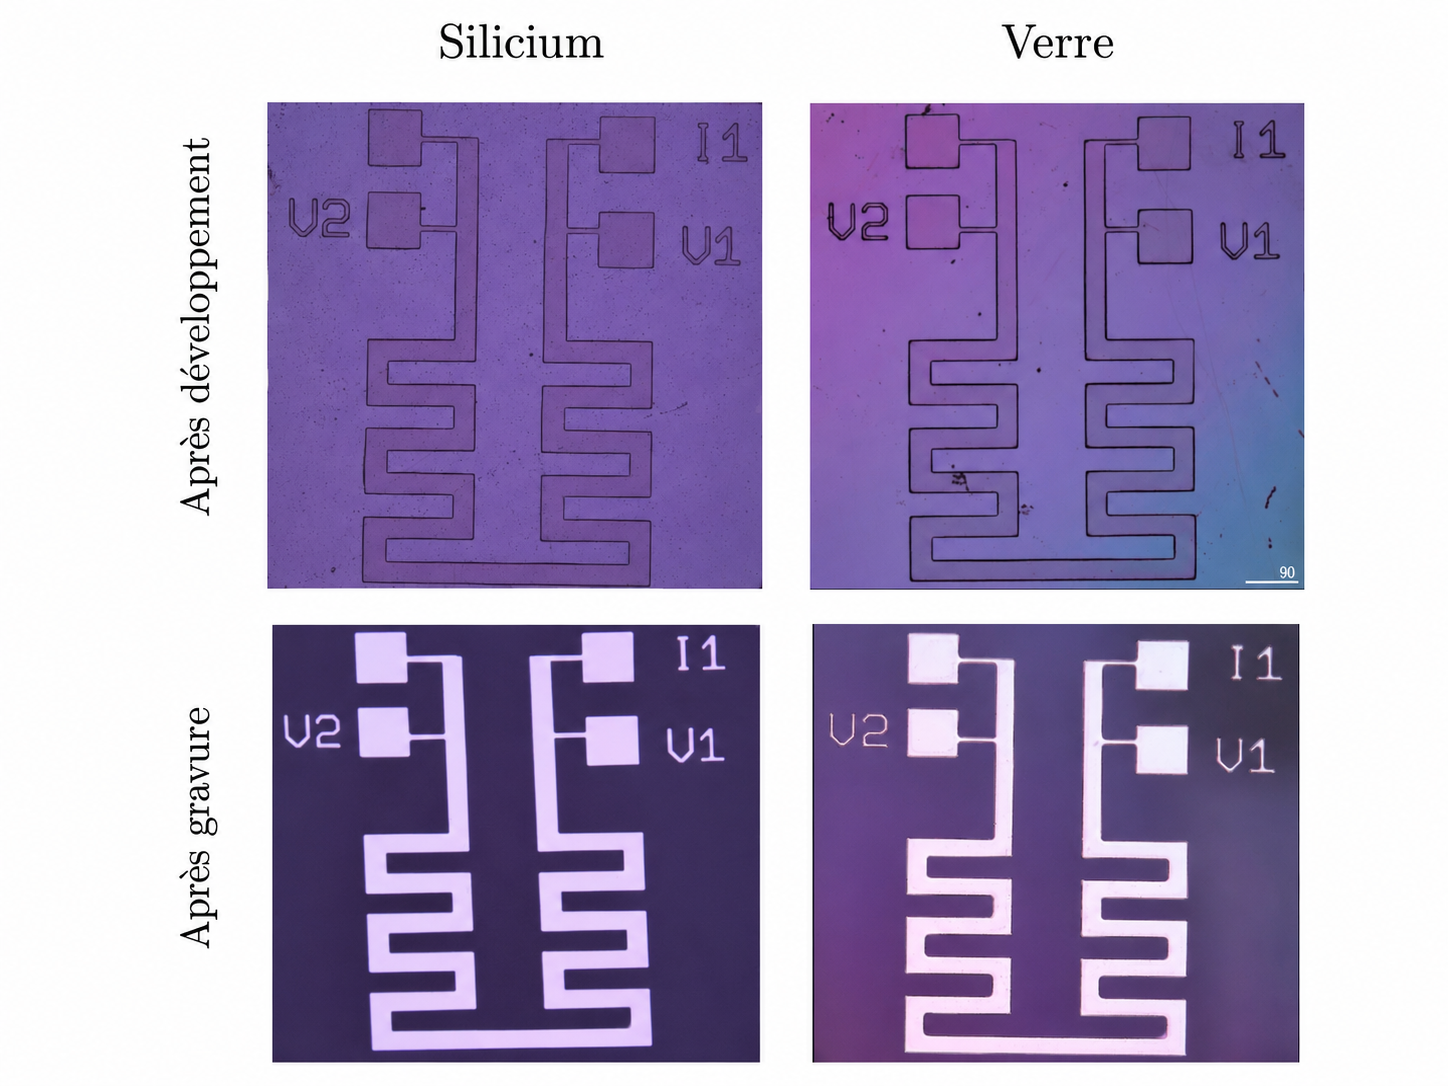
\includegraphics[width=0.72\textwidth]{rapport-micro332/photos/s4_comparaison_gravure.png}
    \caption{Comparaison des motifs observés sur silicium et sur verre.}
    \label{fig:tp4_gravure}
\end{figure}

Sur les deux substrats, les motifs sont bien visibles et les lignes semblent continues. On observe toutefois quelques petits défauts sur les bords des motifs, particulièrement sur les images du verre.

\begin{table}[htbp]
    \centering\small
    \caption{Temps de gravure de l'aluminium mesurés au chronomètre.}
    \label{tab:tp4_gravure}
    \begin{tabular}{@{}lc@{}}
        \toprule
        Substrat & Temps de gravure \\
        \midrule
        Silicium & \qty{4}{\minute}~\qty{13}{\second} \\
        Verre & \qty{4}{\minute}~\qty{37}{\second} \\
        \bottomrule
    \end{tabular}
\end{table}

\noindent\textbf{B. Alignement du photomasque}

L'alignement a été réalisé par chaque binôme sur le même type de wafer en silicium. La figure~\ref{fig:tp4_alignement} présente le repère « 2 » et une croix centrale, photographiés pour chacun des deux binômes.

\begin{figure}[htbp]
    \centering
    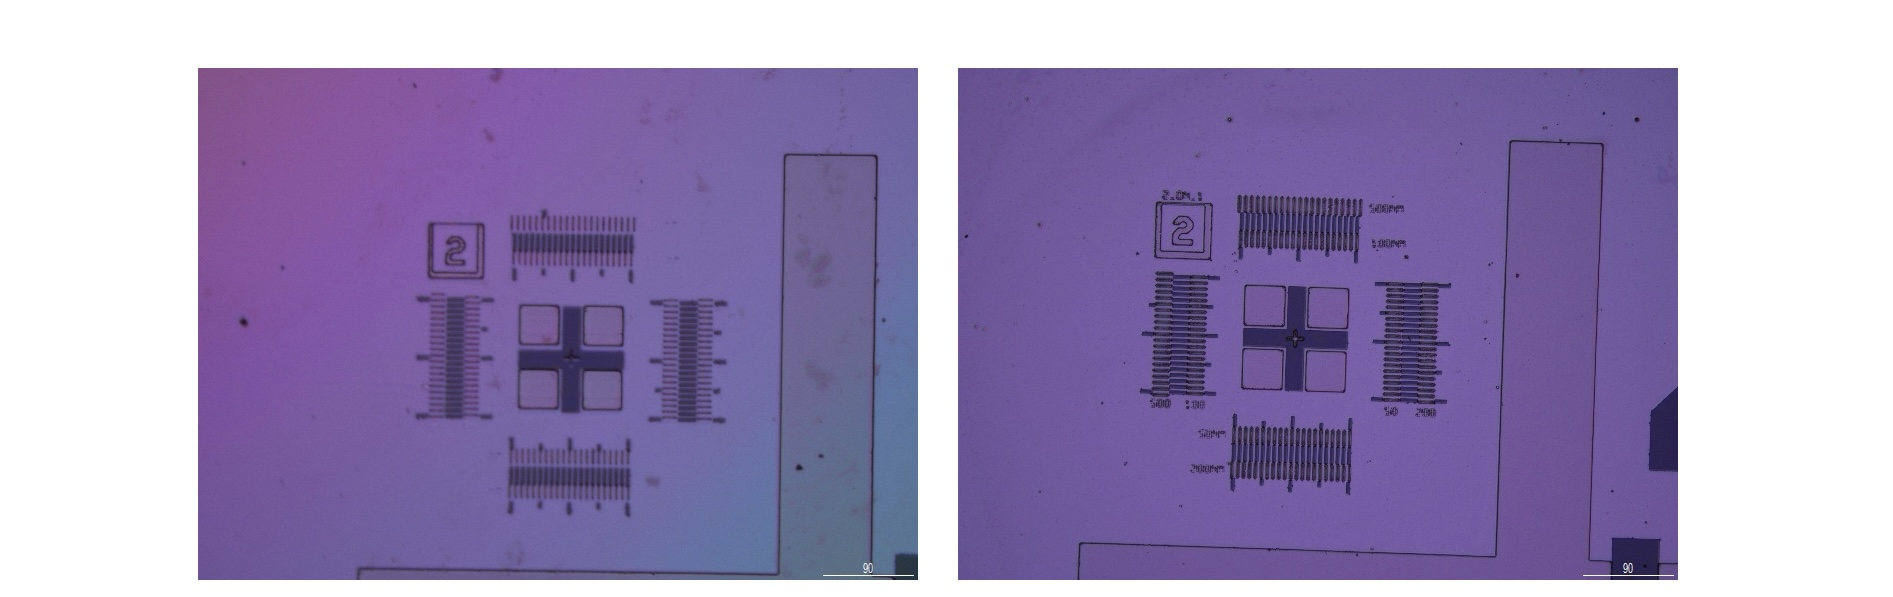
\includegraphics[width=0.72\textwidth]{rapport-micro332/photos/s4_alignement1.jpg}\\[2pt]
    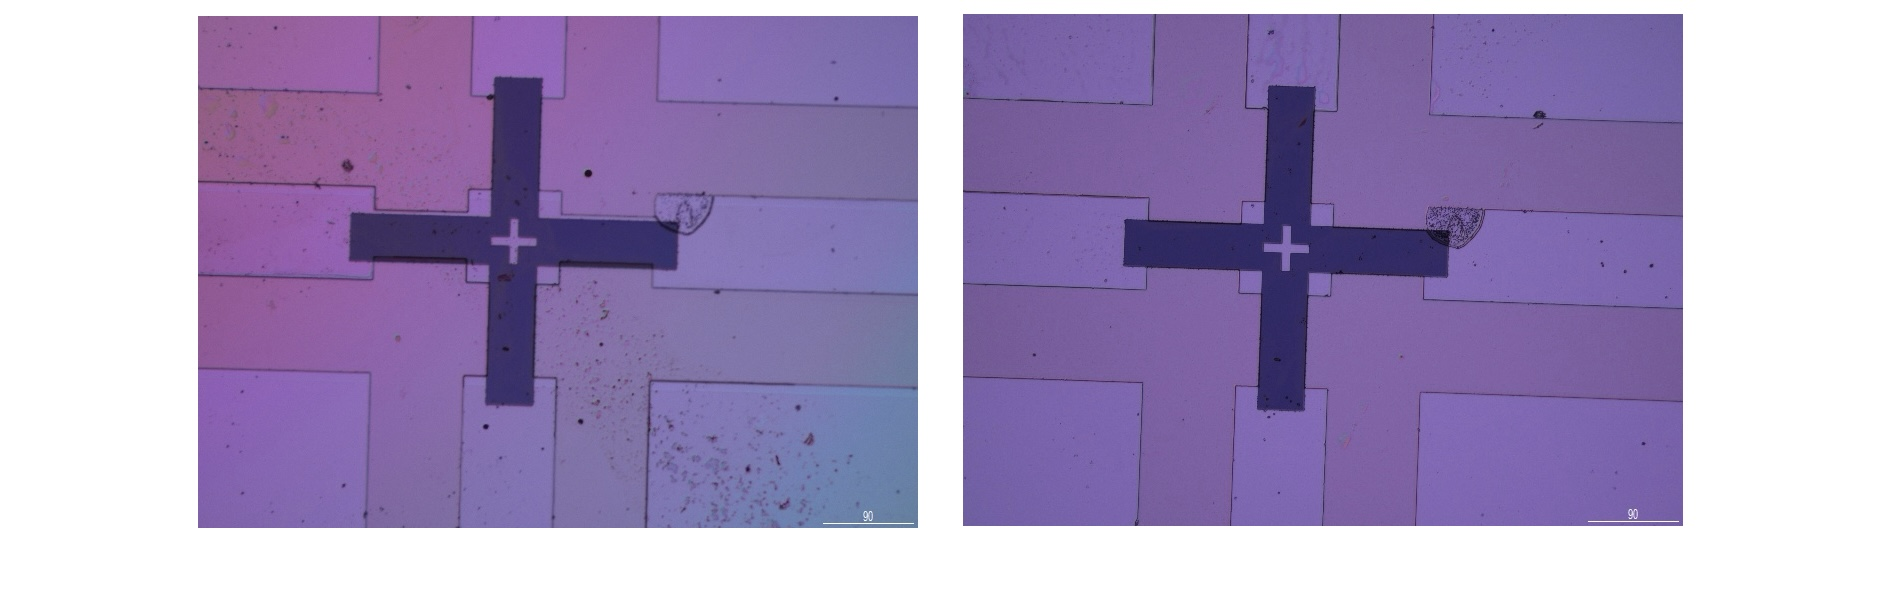
\includegraphics[width=0.72\textwidth]{rapport-micro332/photos/s4_alignement2.jpg}
    \caption{Comparaison des structures après la manipulation d'alignement pour chacun des binômes. En haut : zone de référence « 2 ». En bas : croix centrale.}
    \label{fig:tp4_alignement}
\end{figure}

Dans les deux séries, une croix sombre apparaît autour d'une croix claire, qui sert de repère pour l'alignement visuel des motifs.

\subsection{Analyse}

\noindent\textbf{A. Gravure de l'aluminium}

Les structures obtenues et les temps de gravure sont globalement similaires sur les deux substrats, ce qui indique un transfert réussi des motifs. Les petites imperfections visibles après le développement, probablement dues à des particules ou à des résidus de résine, ne sont plus observables après la gravure.

Les deux temps de gravure (tableau~\ref{tab:tp4_gravure}) diffèrent de \qty{24}{\second}, soit \qty{9}{\percent}. La solution attaque l'aluminium et pas le substrat : à épaisseur d'Al égale, on attend donc des temps proches sur verre et sur silicium. Le temps dépend en revanche surtout de l'épaisseur d'Al, de la température du bain (\qty{40}{\celsius}) et de l'agitation. L'écart restant peut venir d'une différence d'épaisseur entre les deux chips, d'un bain un peu refroidi entre les deux gravures, ou du jugement visuel de la fin de gravure par deux binômes différents, plus délicat sur le verre transparent. La vitesse de gravure de l'Al double environ tous les \qty{5}{\celsius} \cite{alumicro} : un écart de \qty{9}{\percent} correspond à moins de \qty{1}{\celsius} de différence de bain. Le départ de la gravure varie aussi : le développeur attaque déjà l'alumine native là où la résine est ouverte, et les bulles d'hydrogène rendent l'attaque inhomogène \cite{alumicro}. Le protocole demande enfin de comparer la taille d'un même motif avec et sans résine (étape 16) ; nos images ne contiennent pas de cliché du même motif après retrait de la résine, et cette comparaison n'a pas pu être faite.

Les différences visuelles au niveau des contours s'expliquent notamment par les propriétés optiques des substrats. Le silicium, opaque et réfléchissant, offre un contraste plus marqué, tandis que la transparence du verre et les réflexions aux interfaces peuvent rendre les contours moins nets sur les images.
\\

\noindent\textbf{B. Alignement du photomasque}

Les deux alignements sont globalement satisfaisants. On observe toutefois un léger décalage selon l'axe vertical pour l'un des binômes, tandis que l'autre présente une superposition plus précise des croix et de leurs repères. Aucun décalage significatif n'est visible dans ce second cas. Ce jugement reste visuel : nous n'avons pas relevé le décalage en micromètres, ce que permettraient les verniers gradués visibles autour du repère « 2 » (figure~\ref{fig:tp4_alignement}) \cite{prot4}.

\subsection{Conclusion}

Ce sujet a permis de réaliser une gravure sélective de l'aluminium sur deux substrats différents, ainsi que l'alignement d'un photomasque sur des structures préexistantes.
\\

Les résultats montrent que la gravure produit des motifs similaires sur verre et sur silicium, avec des temps de gravure de \qty{4}{\minute}~\qty{13}{\second} et \qty{4}{\minute}~\qty{37}{\second}. Les différences visuelles observées sont probablement liées en partie aux propriétés optiques des substrats.

Enfin, les deux alignements ont été réalisés avec une précision visuellement satisfaisante, malgré un léger décalage observé dans l'un des cas. Ces manipulations illustrent l'importance du contrôle des paramètres de gravure et de la précision de l'alignement en microfabrication.



